%SECCIÓN 3. METODOLOGIA
\section{METODOLOGIA}

 Para el abordar el análisis de este problema se desarrollaran las siguientes tareas [1].
 
  \subsection{Reconocimiento de la información}
 
 El dataset utilizado en este análisis fue obtenido mediante una consulta sobre la base de datos de la Universidad de los Llanos y esta conformada por la información de los estudiantes activos de todas las facultades que componen la universidad.
 
  
  \begin{itemize}
   \item \textbf{Descripción la población}: La población objeto de este análisis esta compuesta por los estudiantes activos (matriculados) de la Universidad de los Llanos, que no poseen problemas académicos o administrativos; se excluyeron los estudiantes que pertenecen a primer semestre de todas las carreras de pregrado, debido a que no poseen promedio ponderado de carrera aún. 
   \bigskip
   La población esta compuesta por los datos de 5000 estudiantes que tiene la Universidad de los Llanos, los cuales fueron obtenidos mediante una consulta a la base de datos del sistema de registro y control académico de la Universidad de los Llanos, de donde se extrajeron en una hoja de calculo los siguientes campos:
   
   \item \textbf{Variables del DataSet:}\\
    
   \begin{itemize}
	   \item \textbf{ciudad}  	: Ciudad de origen del estudiante
	   \item \textbf{dept} 	: Departamento de origen del estudiante
	   \item \textbf{fac\_nac} : Fecha de nacimiento del estudiante
	   \item \textbf{fac\_ing} : Fecha de ingreso del estudiante al programa
	   \item \textbf{estrato}	: Estrato socieconomico del estudiante
	   \item \textbf{promedio} : Promedio ponderado de carrera del estudiante
	   \item \textbf{carrera}  : Programa académico que cursa el estudiante
	   \item \textbf{codigo}   : Código del estudiante
	   \item \textbf{nombre}   : Nombres y apellidos del estudiante
	   \item \textbf{identificacion}: Numero de identificación del estudiante
	\end{itemize}
   
    \item \textbf{Identificación del problema}: Determinar si la situación socio económica (estrato socio económico) puede generar consecuencias directas sobre el rendimiento académico de los estudiantes de la Universidad de los Llanos\\ 
    
   \item \textbf{Objetivos}: El objetivo de este análisis es determinar si el estrato socioeconomico incide en el rendimiento académico de los estudiantes de la Universidad de los Llanos.
  \end{itemize}
  \subsection{Preguntas de investigación}
  Las preguntas de investigación que se abordan en este análisis son las siguientes:
  \begin{itemize}
   \item ¿Existe algún tipo de relación entre el estrato socio económico y el desarrollo intelectual?
   \item ¿Los estudiantes falsean el estrato social real, para obtener beneficios económicos en el valor de la matricula?
   \item ¿La elección de estudiar en la Universidad de los Llanos, se realiza para reducir costos?
   \item ¿La elección de estudiar en la Universidad de los Llanos, se realiza para obtener reconocimiento académico de la misma?
  \end{itemize}
  \subsection{Análisis exploratorio}
  
  	Las variables que son objeto del análisis en esta investigación son el estrato socieconomico y el promedio ponderado de carrera, a continuación se realiza el análisis de cada una de ellas:
  
  \begin{itemize}
  	%alzate
	\item \textbf {Variable Estrato Socioeconomico}: Esta variable es un atributo de carácter ordinal, a la cual se le puede aplicar la moda como medida de tendencia central y utilizar el diagrama de sectores o torta como forma de representación gráfica con el fin de establecer la distribución de cada estrato respecto al total de la población.  \\
	
	Los datos utilizados para analizar el comportamiento de la variable estrato socieconomico se resumen en la tabla que se muestra a continuación:
	 \bigskip
	\begin{figure} [ht]
		\centering
		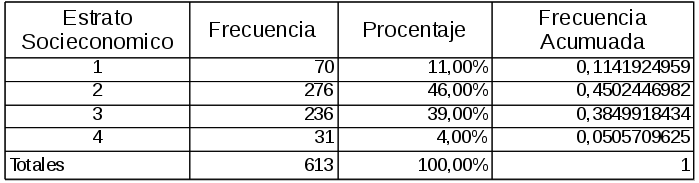
\includegraphics[width=1\linewidth]{figure/cuadro_socioeconomico}
		\caption{Variable Estrato Socioeconomico}
		\label{fig:cuadro_socioeconomico}
	\end{figure}

	Representaciones gráfica de la población por estrato utilizando diagramas de sectores o torta:  

	\begin{figure} [ht]
		\centering
		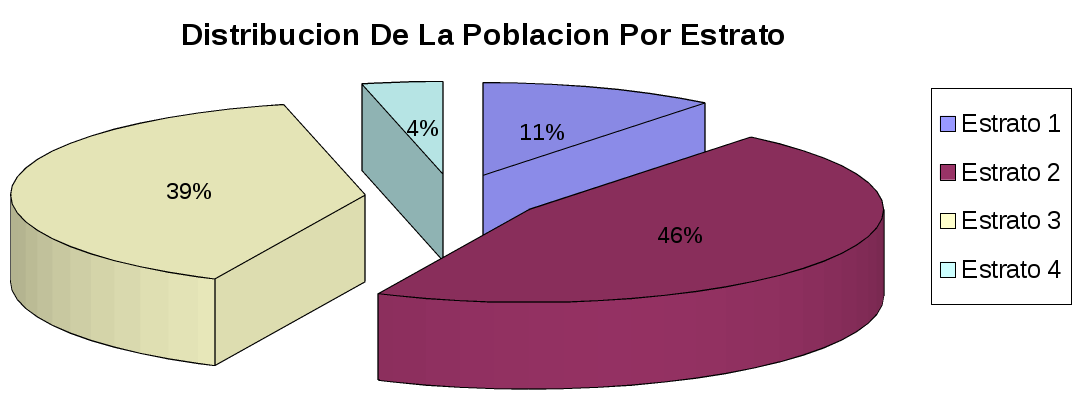
\includegraphics[width=0.9\linewidth]{figure/diagrama_sectores}
		\caption{Diagrama de sectores}
		\label{fig:diagrama_sectores}
	\end{figure}

	Como se puede observar en el anterior diagrama de sectores la mayor cantidad de observaciones se encuentran agrupadas en el estrato 2 con un porcentaje de ocurrencia del 46\%.\\
	   
	Como se puede observar en el siguiente diagrama de barras la mayor cantidad de observaciones en la población ocurren en el estrato 2 con una frecuencia de 275 que corresponde al estrato hacia el que tienden a agruparsen las observaciones.
   \bigskip
	\begin{figure}[ht]
		\centering
		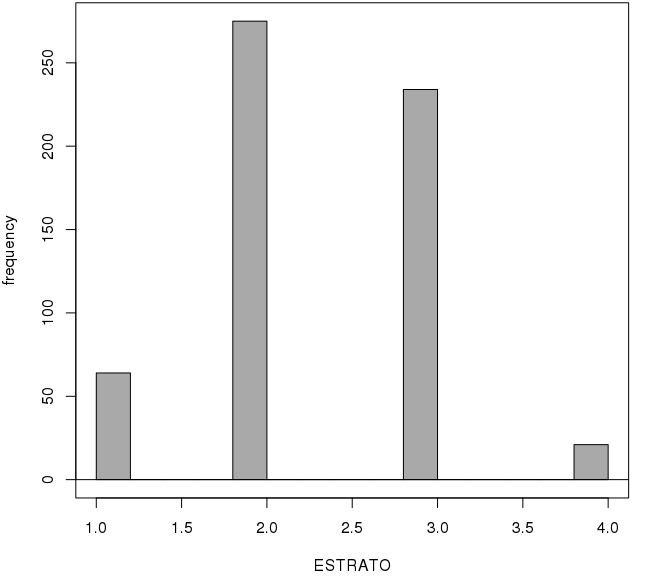
\includegraphics[width=0.7\linewidth]{figure/diagrama_barras}
		\caption{Diagrama de barras}
		\label{fig:diagrama_barras}
	\end{figure}

  	\item \textbf {Variable Promedio Ponderado de Carrera:}
		El promedio ponderado de carrera es una variable de carácter cuantitativo de tipo continuo en la que se utilizaron cinco intervalos para analizar el comportamiento de los 613 promedios de carrera de los estudiantes de pregrado de la Universidad de los Llanos.
   \bigskip
	\begin{itemize}
		\item Intervalo 1: promedios de carrera entre 0 y 1  
		\item Intervalo 2: promedios de carrera entre 0,1 y 2
		\item Intervalo 3: promedios de carrera entre 2,1 y 3
		\item Intervalo 4: promedios de carrera entre 3,1 y 4 
		\item Intervalo 5: promedios de carrera entre 4,1 y 5
	\end{itemize}
	\bigskip
	Los datos utilizados para analizar el comportamiento de la variable promedio ponderado de carrera se resumen en la tabla que se muestra a continuación:
	\bigskip
	
	\begin{figure}[ht]
		\centering
		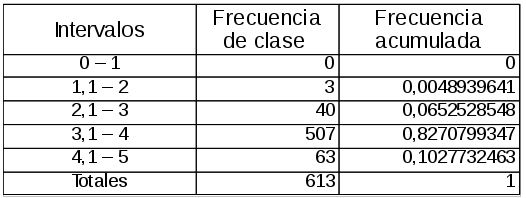
\includegraphics[width=0.7\linewidth]{figure/cuadro_promedio}
		\caption{Variable Promedio Ponderado de Carrera}
		\label{fig:cuadro_promedio}
	\end{figure}

	Representación gráfica de la variable promedio ponderado de carrera utilizando diagrama de barras para analizar el comportamiento en un histograma de frecuencias relativas.

	\begin{figure}[ht]
		\centering
		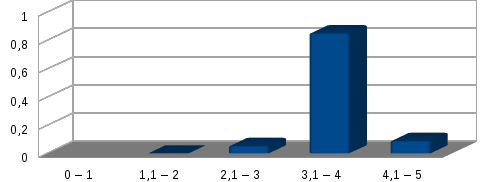
\includegraphics[width=0.9\linewidth]{figure/diagrama_barras_promedio}
		\caption{Histograma Frecuencias Relativas}
		\label{fig:diagrama_barras_promedio}
	\end{figure}

	Representación gráfica de la variable promedio ponderado de carrera utilizando diagrama de barras para analizar el comportamiento en un histograma con frecuencias de clase.

	\begin{figure}[ht]
		\centering
		<<echo=false, fig=true>>=
			with(datosep, hist(promedio, breaks="Sturges", col="darkgray", main="Histograma de frecuencias de clases"))
		@
		\caption{Histograma Frecuencias de Clases}
		\label{fig:barras_promedio_frecuencias_clase}
	\end{figure}



  	\item \textbf {Diseño del espacio muestral:}
	El muestreo aplicado para abordar el análisis de este problema es Muestreo Aleatorio Simple (MAS) y el método utilizado para realizar la selección de los datos que conforman la muestra es coordinado negativo.
	
		
	\bigskip
	Los datos introducidos en los parámetros que proporciona la plantilla (documento adjunto) para calcular el tamaño de la muestra utilizando Muestreo Aleatorio Simple MAS, son los que se muestran a continuación:\\
	
	\begin{itemize}
		\item Tamaño de la población 	N = 5000	
		\item Error que se comete		E = 0,03	\\se recomienda que este entre 0,02 y 0,03
		\item Proporción del dominio	P = 0,02	\\P tomar valores entre 0 y 1
		\item Nivel de confianza		C = 0,95	\\(1 – alfa) donde alfa toma valores entre (0 y 1)
	\end{itemize}
	\bigskip
  	  	El tamaño de la muestra después de aplicar la técnica del coordinador negativo (M) es:
  	\bigskip  	
  	\begin{itemize}
  		\item Variabilidad			V = 0,0196329966
	  	\item Valor del percentil 	Z(alfa) = -1,959963985
		\item Tamaño de la muestra 	M = 613  	
  	\end{itemize}
  	\bigskip  	
  	Una vez obtenido el tamaño de la muestra, se aplico la técnica de coordinador negativo, a los datos de los estudiantes que se encuentran almacenados en la hoja de calculo; el procedimiento realizado es el que se describe a continuación:
  	\bigskip
  	\begin{itemize}
  		\item Asigna un numero aleatorio a cada dato de la muestra
		\item Se ordena de menor a mayor con respecto a la asignación aleatoria 
		\item Se selecciona del primero hasta el tamaño de la muestra  
  	 \end{itemize}
  	\bigskip  		
  	Para el caso de los estudiantes de la Universidad de los Llanos se poseen los datos completos de toda la población objeto de análisis, pero con fin de mostrar el proceso de calcular el tamaño de la muestra y realizar de forma correcta la estimación bajo criterios de normalidad se selecciono una muestra de tamaño 613.
  	
%canavos
   
   \item Medidas de tendencia central[4] 
	   \begin{itemize}
		 	\item Media: la media de las observaciones de un experimento aleatorio $x_{1},x_{2},.....x_{n}$ es el promedio aritm\'etrico de \'estas y se denota por;
		 	$$\overline{x}=\sum_{i=1}^{n} \frac{X_{i}}{n}$$ 
		 	\item Moda: la moda de un conjunto de observaciones de un experimento aleatorio es elvalor de la observaci\'on que ocurre con mayor frecuencia en el conjunto.
		 	%14
		 	\item Mediana: la mediana representa el valor de la variable de posición central en un conjunto de datos ordenados de un experimento aleatorio.
		 \end{itemize}
		 
		 
		 %15\
		 \item Varianza [4] : La Varianza de las observaciones $x_{1},x_{2},...,x_{n}$ es en esencia, el promedio del cuadrado de las distancias entre cada observaci\'on y la media del conjunto de observaciones. Se denota por:
		 $$s^{2}=\sum_{i=1}^{n} \frac{ \left( x_{i}-\overline{x}\right)^{2}}{\left(n-1 \right) } $$ 
		 
		 
		 \item Desviación estándar [4]: La desviaci\'on est\'andar es la raiz cuadrada de la varianza y se denota por:
		 $$s=\sqrt{\sum_{i=1}^{n} \frac{ \left( x_{i}-\overline{x}\right)^{2}}{\left(n-1 \right) } }$$ 
		 
		 
		 
		 Se puede aplicar una medida de tendencia central como la media y un medida de dispersión  como la varianza. A continuación se muestran los valores calculados para la variable promedio de carrera ponderado.
		 \begin{figure}[ht]
			\centering
			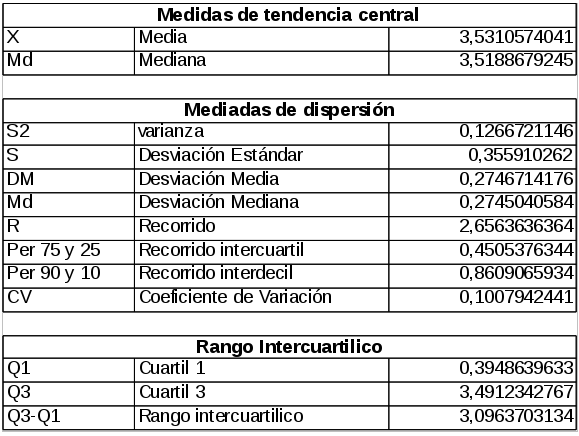
\includegraphics[width=0.9\linewidth]{figure/medidas_rpbabilidad}
			\caption{}
			\label{fig:medidas_rpbabilidad}
		\end{figure}

 
\end{itemize}  



